\chapter{User API}
\label{chap:design}
TimeKeeper comes with a simple and intuitive set of functions to create and manage time-dilated containers. The presented API describe the set of functions TimeKeeper provides to the user. The functions are defined in scripts/TimeKeeper\_functions.h. You can ignore this section if you are going to use TimeKeeper with the CORE or ns-3 modifications, as everything is handled internally.

\section{General Functions}
\begin{description}
 \item[clone\_time(unsigned long flags, float dilation, int should start) ] \hfill \\
 The $clone\_time()$ function will cause a new process to be cloned from the calling process. The $flags$ argument is a bitmap of various tunable knobs similar to the $clone()$ system call. The $dilation$ argument represents the dilation factor of this new process. The $should\_start$ argument determines if the new time-dilated process should be allowed to start running immediately or not. A $should\_start$ value of 0 means the process will immediately start, while a $should\_start$ value of 1 means the new process should not immediately start. Not immediately starting a new process may be useful if you wish to clone numerous time-dilated processes, but need them all to start running at the same point in physical time (as you may need to do in an $experiment$).
 \item[dilate(int pid, float dilation) ] \hfill \\
 The $dilate()$ function will change the TDF of a process. The $pid$ argument represents the unique process identifier of the process whose TDF you wish to change. The $dilation$ argument represents the new dilation factor of the process. This function can be called on both a process that was instantiated through the $clone\_time()$ function, as well as any standard Linux process.
 \item[dilate\_all(int pid, float dilation) ] \hfill \\
The $dilate\_all()$ function will do the same thing as the $dilate()$ function, but in addition will recursively set the TDF of every child and grandchild of the process. 
 \item[freeze(int pid)] \hfill \\
The $freeze()$ function will stop a process from continuing to execute on the processor. The current system time in which it was frozen is stored in the process's corresponding $task\_struct$.
\item[freeze\_all(int pid) ] \hfill \\
The $freeze\_all()$ function will do the same thing as the $freeze()$ function, but in addition will recursively freeze every child and grandchild of the process. 
 \item[unfreeze(int pid) ] \hfill \\
The $unfreeze()$ function allows a previously frozen process to be unfrozen and continue execution. In between the time in which the process was frozen and unfrozen, the process will not perceive any passage of time. For example, if a process was frozen at time 30 seconds, and unfrozen at time 40 seconds, it will resume its execution at time 30 seconds. 
\item[unfreeze\_all(int pid) ] \hfill \\
The $unfreeze\_all()$ function will do the same thing as the $unfreeze()$ function, but in addition will recursively unfreeze every child and grandchild of the process. 
\item[leap(int pid, int otherPid) ] \hfill \\
The $leap()$ function changes the process's virtual time specified by $pid$ to be identical to that of the process with the given id $otherPid$. When this is applied to a process that is currently frozen, the process will essentially leap over an epoch of virtual time, without needing to directly modify its TDF. 
\item[gettimepid(int pid, struct timeval tv, struct timezone tz) ] \hfill \\
The $gettimepid()$ function will query the current virtual time of the process specified by the $pid$. This can be queried on a process with a TDF or without a TDF.
\item[gettimename(char *lxcname, struct timeval tv, struct timezone tz) ] \hfill \\
The $gettimename()$ function is the same as the $gettimepid()$ function, but it takes an LXC name instead of a $pid$. 
\item[gettimeofdayoriginal(struct timeval tv, struct timezone tz) ] \hfill \\
The $gettimeofdayoriginal()$ function will return the actual system time, regardless of whether the calling process is time-dilated or not. This is useful mainly for debugging, when you want to verify the virtual time is being scaled appropriately with respect to the system time.
\end{description}
\begin{figure}[t] 
      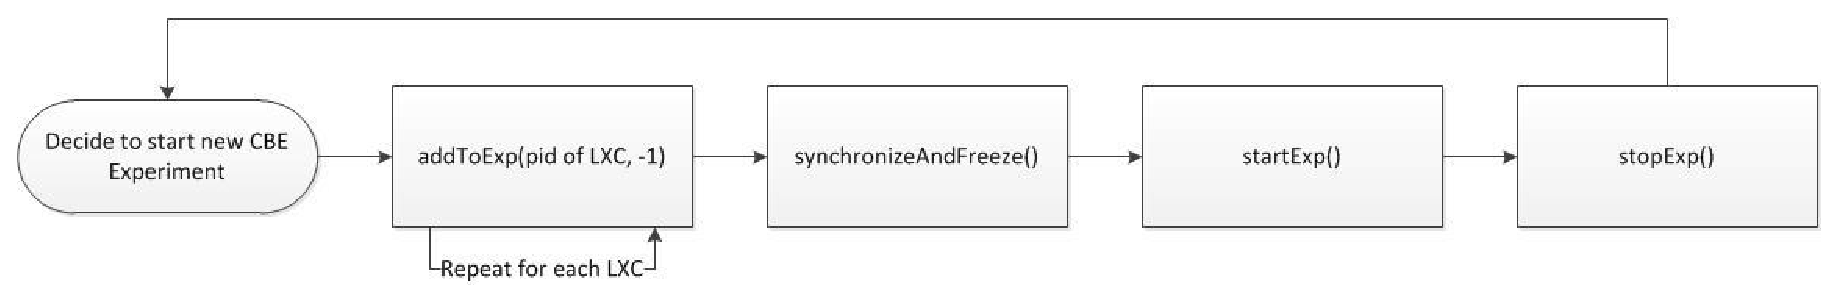
\includegraphics[width=\textwidth]{images/cbe_functions.eps} 
    \caption{Order of Operations to Setup a CBE Experiment } 
    \label{fig:cbe_functions} 
  \end{figure} 
\begin{figure}[t] 
      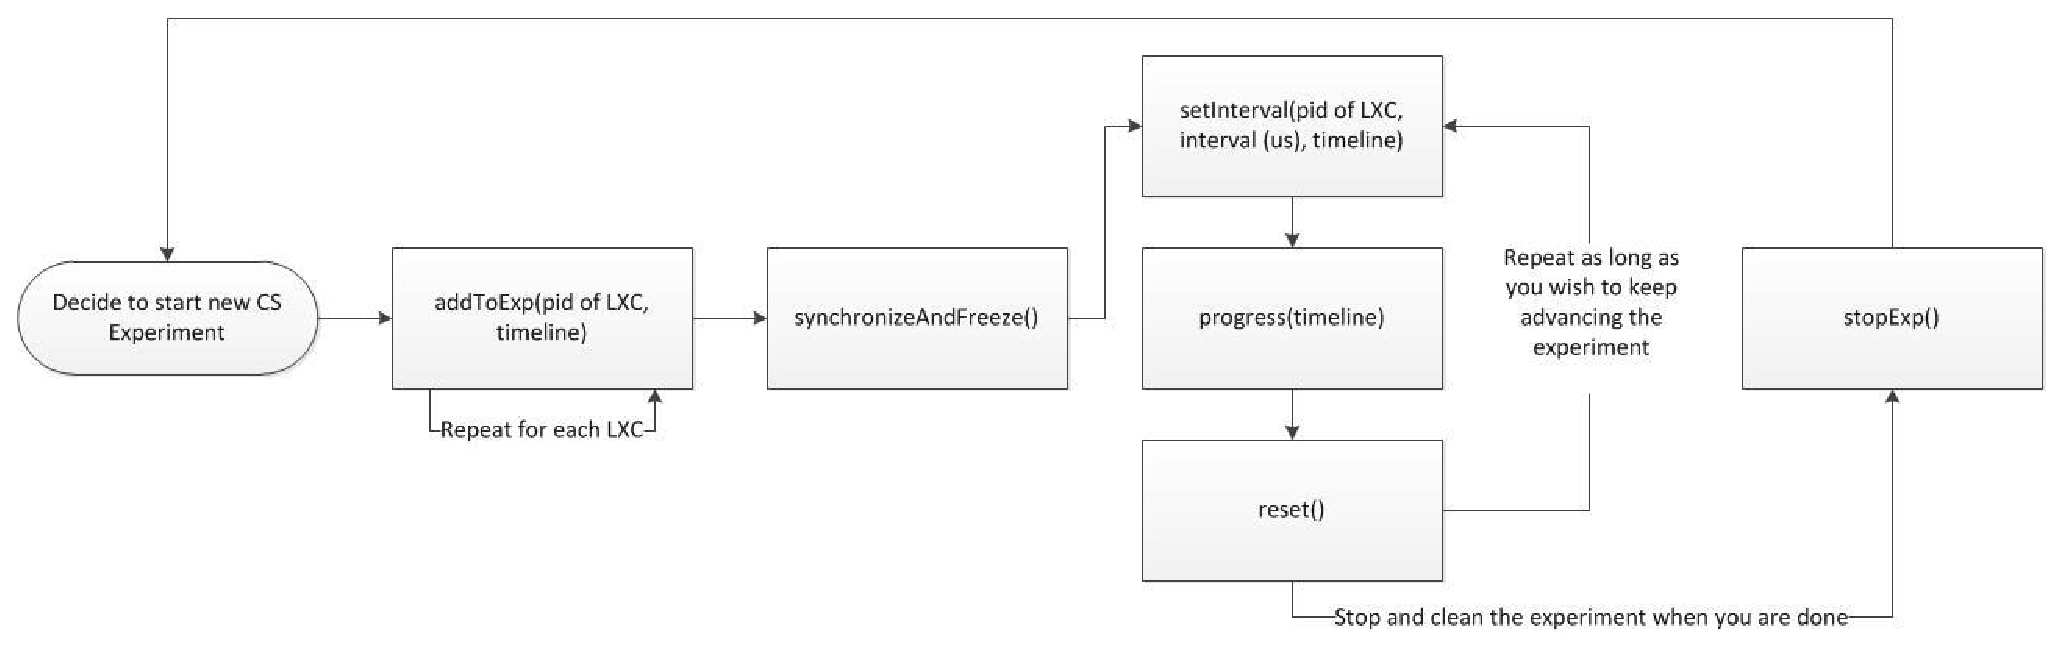
\includegraphics[width=\textwidth]{images/cs_functions.eps} 
    \caption{Order of Operations to Setup a CS Experiment } 
    \label{fig:cs_functions} 
  \end{figure} 
\section{Experiment Synchronization Methods}
TimeKeeper supports two methods to perform experiment synchronization. They are discussed below.
\subsection{Concurrent Best Effort}
Concurrent Best Effort (CBE) is when the emulated nodes and the network simulator run side by side. The network simulator is tied to some external clock (usually the system clock), and advances at the same rate as the emulated nodes. The simulator will make a best effort to deliver packets when it should. If a packet is too late, the simulator may send the packet as soon as it can, or simply drop the packet. In a CBE experiment, the simulator is not aware of TimeKeeper, and does not need to directly interact with it. Any experiments conducted with the CORE or ns-3 simulator utilizes the CBE method.
\subsection{Concurrent Synchronization}
With Concurrent Synchronization (CS) the simulator directly communicates with TimeKeeper, and specifies how far each LXC's virtual time should be allowed to advance in the following round. When the round is started, the simulator executes all events within that interval (the current virtual time and the virtual time to which each LXC will advance to). At the end of each round, the simulator may respecify how far each LXC can progress in virtual time, then start a new round. The CS method was utilized when TimeKeeper was integrated with S3F.

\section{Experiment Synchronization Functions}
The following functions were developed to support both CBE and CS experiments. The order of operations to perform a CBE experiment is outlined in Figure \ref{fig:cbe_functions}, while the order of operations to perform a CS experiment is outlined in Figure \ref{fig:cs_functions}. You should be careful and try not to mix functions (trying to call both $startExp()$ and $setInterval()$ in the same experiment), as this may give inaccurate results.
\begin{description}
\item[addToExp(int pid, int timeline) ] \hfill \\
The $addToExp()$ function call will add the given $pid$ of the LXC to the experiment. If a $timeline$ is supplied, it means you are going to try to start a CS experiment. If $timeline$ is less than 0, you will be setting up a CBE experiment. 
\item[synchronizeAndFreeze() ] \hfill \\
Once all of the LXCs have been added to the experiment, the $synchronizeAndFreeze()$ function is called, which will freeze all of the LXCs, and set all of their virtual times to be at the same starting point. 
\item[startExp()] \hfill \\
The $startExp()$ function will start a synchronized experiment with TimeKeeper. The prerequisite functions of $addToExp()$ and $synchronizeAndFreeze()$ are necessary before calling this function.
\item[setInterval(int pid, int interval, int timeline) ] \hfill \\
The $setInterval()$ function will specify the interval in which you wish an LXC will advance in virtual time. The $pid$ represents the $pid$ of the LXC, $interval$ represents the virtual time advancement in microseconds, and the $timeline$ value must correspond to the timeline associated with the LXC. 
\item[progress(int timeline, int force) ] \hfill \\
The $progress()$ function will progress all LXC's virtual times by the amount specified by the $setInterval()$ function and associated with the given $timeline$. If an LXC has not been assigned an interval with the $setInterval()$ function, then its virtual time will not progress. The function will return when all LXCs associated with the given $timeline$ had advanced to the correct virtual time. If $force$ is 0, then TimeKeeper will do a best effort to bring each LXC to the correct virtual time. However, there may be a certain amount of error, as the underlying mechanism for freezing and unfreezing is not 100\% accurate. If $force$ is 1, each LXC's virtual time will progress to precisely the exact moment in virtual time in which it should. This is done by changing each LXC's virtual time after it is frozen.
\item[reset(int timeline) ] \hfill \\
The $reset()$ function will reset all previously set intervals for all LXCs on the given $timeline$. 
\item[stopExp()] \hfill \\
The $stopExp()$ function call will stop a running experiment. This will be used after the experiment has finished, and you wish to clean up TimeKeeper. Once TimeKeeper is cleansed with this function, you may proceed to set up a new experiment.
\end{description}

\section{Utility Scripts}
In addition to the API, simple utility scripts were created to perform TimeKeeper commands from the command line. They are located in /path/to/TimeKeeper/scripts.
\begin{description}
 \item \textbf{timekeeper-dilate [-r] [-p pid] [-n name] TDF} \hfill \\
	Sets the TDF of a process. -r dilates all children of the process as well. You may use either -p to specify a pid, or -n to specify the LXC name. 
 \item \textbf{timekeeper-freeze [-r] pid} \hfill \\
	Freezes a process specifed by pid. -r will freeze all children of the process as well.
 \item \textbf{timekeeper-unfreeze [-r] pid} \hfill \\
	Unfreezes a process specifed by pid. -r will unfreeze all children of the process as well.
 \item \textbf{timekeeper-gettime [-p pid] [-n name]} \hfill \\
	Returns the current time of a process. You may use either -p to specify a pid, or -n to specify the LXC name. 

 \item \textbf{timekeeper-addToExperiment [-t timeline] [-d tdf] [-p pid] [-n name]} \hfill \\
	Adds a process to an experiment. You may use -t to specify a timeline, and -d to specify a TDF. You may use either -p to specify a pid, or -n to specify the LXC name.
 \item \textbf{timekeeper-synchronizeAndFreeze} \hfill \\
	Will freeze all of the processes added to the experiment, and set their virtual times to be the same
 \item \textbf{timekeeper-startExperiment} \hfill \\
	Starts a CBE experiment.
 \item \textbf{timekeeper-setInterval [-p pid] [-n name] TIMEus timeline} \hfill \\
	Sets the virtual time progression of a process. You may use either -p to specify a pid, or -n to specify the LXC name. The TIME is in microseconds. 
 \item \textbf{timekeeper-progress [-f] [-t timeline]} \hfill \\
	Progresses all LXCs associated with the specified timeline. -f flag will force the process to advance at the exact interval. 
 \item \textbf{timekeeper-reset [-t timeline]} \hfill \\
        Resets all progression interviews associated with a timeline
 \item \textbf{timekeeper-stopExperiment} \hfill \\
	Stops an experiment
\end{description}
